\documentclass[tikz,border=10pt]{standalone}
\usepackage{tikz}
\usetikzlibrary{positioning, shapes, arrows.meta}

\begin{document}
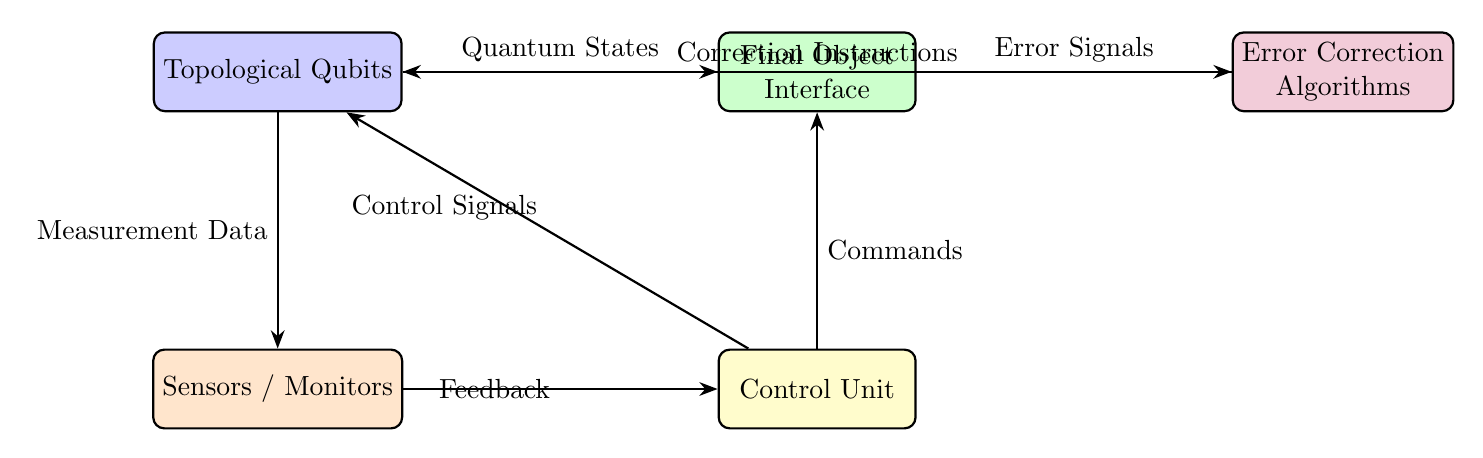
\begin{tikzpicture}[node distance=2.5cm, auto, thick,
    block/.style={draw, rectangle, rounded corners, minimum width=2.5cm, minimum height=1cm, align=center},
    arrow/.style={-{Stealth[scale=1.0]}, thick}]

    % Nodes
    \node[block, fill=blue!20] (tq) {Topological Qubits};
    \node[block, fill=green!20, right=4cm of tq] (interface) {Final Object\\Interface};
    \node[block, fill=orange!20, below=3cm of tq] (sensors) {Sensors / Monitors};
    \node[block, fill=yellow!20, below=3cm of interface] (control) {Control Unit};
    \node[block, fill=purple!20, right=4cm of interface] (algorithms) {Error Correction\\Algorithms};

    % Arrows
    \draw[arrow] (tq) -- node[above] {Quantum States} (interface);
    \draw[arrow] (tq) -- node[left] {Measurement Data} (sensors);
    \draw[arrow] (interface) -- node[above] {Error Signals} (algorithms);
    \draw[arrow] (sensors) -- node[left] {Feedback} (control);
    \draw[arrow] (control) -- node[above left] {Control Signals} (tq);
    \draw[arrow] (algorithms) -- node[above] {Correction Instructions} (tq);
    \draw[arrow] (control) -- node[below right] {Commands} (interface);
\end{tikzpicture}
\end{document}
